% This is "sig-alternate.tex" V2.0 May 2012
% This file should be compiled with V2.5 of "sig-alternate.cls" May 2012
%
% This example file demonstrates the use of the 'sig-alternate.cls'
% V2.5 LaTeX2e document class file. It is for those submitting
% articles to ACM Conference Proceedings WHO DO NOT WISH TO
% STRICTLY ADHERE TO THE SIGS (PUBS-BOARD-ENDORSED) STYLE.
% The 'sig-alternate.cls' file will produce a similar-looking,
% albeit, 'tighter' paper resulting in, invariably, fewer pages.
%
% ----------------------------------------------------------------------------------------------------------------
% This .tex file (and associated .cls V2.5) produces:
%       1) The Permission Statement
%       2) The Conference (location) Info information
%       3) The Copyright Line with ACM data
%       4) NO page numbers
%
% as against the acm_proc_article-sp.cls file which
% DOES NOT produce 1) thru' 3) above.
%
% Using 'sig-alternate.cls' you have control, however, from within
% the source .tex file, over both the CopyrightYear
% (defaulted to 200X) and the ACM Copyright Data
% (defaulted to X-XXXXX-XX-X/XX/XX).
% e.g.
% \CopyrightYear{2007} will cause 2007 to appear in the copyright line.
% \crdata{0-12345-67-8/90/12} will cause 0-12345-67-8/90/12 to appear in the copyright line.
%
% ---------------------------------------------------------------------------------------------------------------
% This .tex source is an example which *does* use
% the .bib file (from which the .bbl file % is produced).
% REMEMBER HOWEVER: After having produced the .bbl file,
% and prior to final submission, you *NEED* to 'insert'
% your .bbl file into your source .tex file so as to provide
% ONE 'self-contained' source file.
%
% ================= IF YOU HAVE QUESTIONS =======================
% Questions regarding the SIGS styles, SIGS policies and
% procedures, Conferences etc. should be sent to
% Adrienne Griscti (griscti@acm.org)
%
% Technical questions _only_ to
% Gerald Murray (murray@hq.acm.org)
% ===============================================================
%
% For tracking purposes - this is V2.0 - May 2012

\documentclass{sig-alternate}
\graphicspath{ {images/} }

\usepackage{float}
\usepackage{nameref}

\begin{document}

\title{Classification of Information From Issue Tracking Systems}
\subtitle{[Proposal]}
%
% You need the command \numberofauthors to handle the 'placement
% and alignment' of the authors beneath the title.
%
% For aesthetic reasons, we recommend 'three authors at a time'
% i.e. three 'name/affiliation blocks' be placed beneath the title.
%
% NOTE: You are NOT restricted in how many 'rows' of
% "name/affiliations" may appear. We just ask that you restrict
% the number of 'columns' to three.
%
% Because of the available 'opening page real-estate'
% we ask you to refrain from putting more than six authors
% (two rows with three columns) beneath the article title.
% More than six makes the first-page appear very cluttered indeed.
%
% Use the \alignauthor commands to handle the names
% and affiliations for an 'aesthetic maximum' of six authors.
% Add names, affiliations, addresses for
% the seventh etc. author(s) as the argument for the
% \additionalauthors command.
% These 'additional authors' will be output/set for you
% without further effort on your part as the last section in
% the body of your article BEFORE References or any Appendices.

\numberofauthors{6} %  in this sample file, there are a *total*
% of EIGHT authors. SIX appear on the 'first-page' (for formatting
% reasons) and the remaining two appear in the \additionalauthors section.
%
\author{
% You can go ahead and credit any number of authors here,
% e.g. one 'row of three' or two rows (consisting of one row of three
% and a second row of one, two or three).
%
% The command \alignauthor (no curly braces needed) should
% precede each author name, affiliation/snail-mail address and
% e-mail address. Additionally, tag each line of
% affiliation/address with \affaddr, and tag the
% e-mail address with \email.
%
% 1st. author
\alignauthor
Benedikt Kersjes
% 2nd. author
\alignauthor
Bernhard Wetzel
% 3rd. author
\alignauthor 
Christopher V{\"o}lker
\and  % use '\and' if you need 'another row' of author names
% 4th. author
\alignauthor
Gerd Matheis
% 5th. author
\alignauthor 
Marvin Wyrich
% 6th. author
\alignauthor 
Nazli Olcay Kaya
\and
% 7th. author
\alignauthor 
Steven Gro{\ss}mann
}
% There's nothing stopping you putting the seventh, eighth, etc.
% author on the opening page (as the 'third row') but we ask,
% for aesthetic reasons that you place these 'additional authors'
% in the \additional authors block, viz.

% Just remember to make sure that the TOTAL number of authors
% is the number that will appear on the first page PLUS the
% number that will appear in the \additionalauthors section.

\maketitle

\begin{abstract}
\textit{
The proper management of software is essential for the success of a development project. Hence, version control systems and issue trackers are used to manage and document the evolution of the project. Commit messages of version control systems, issue descriptions and titles of issue tracking systems are written in natural language. Therefore, the information can be classified by using natural language processing. Known data classification techniques like e.g. Naive Bayes, K nearest, etc. can additionally help to analyze further information of software management tools, like meta data. 
In this paper we want to analyze whether it is possible to connect commit messages and issues. For that purpose we developed and implemented an analyzation method. We used data from an academic software project to verify the effectiveness of our developed approach. 
We found out that it is essential to have a high quality of the commit messages, i.e. the commits have to be well formatted according to commit standards. Otherwise the method is not able to work accurate.}
\end{abstract}

\section{Introduction}
\label{sec:introduction}
%Einleitung
%Warum ist das Thema wichtig?
%Wo wirds benötigt oder eingesetzt?
%Welche Fragen sollen beantwortet werden?

For software development projects it is essential to use proper software tools to manage historical information of a project \cite{fischer2003populating}. The use of version control systems like SVN, Git, Mercurial, etc. provide features to track changes on the developed software. Changes on software are made to upgrade, fix or replace parts of the software to improve the overall system \cite{janak2009issue}. However, changes do not always fulfill the intended goal of improving the system or get deprecated after some time. Therefore, it is important to collect information about all changes committed in a repository. The information that can be extracted of version control systems are e.g. change rates, error proneness or starvation of the software project \cite{fischer2003populating}. This can help to understand the evolution of the project to learn from past development mistakes and improve the development in the future.

The software changes in a project are based on specific issues like error reports, feature requests or requirement changes. Those issues can be tracked by bug repositories or issue tracking systems \cite{fischer2003populating}. Especially in the past years, there is an increasing attention of reporting bugs in issue tracking systems \cite{ahmedpredicting}. This is a positive evolution, as developers get active feedback of users and testers, which can result in a faster elimination of problems. 
Every issue in such a management tool contains specific meta information about the problem that has to be solved. I.e. for example a description of the problem, the time to solve the issue and an impact analysis, meaning a possible solution to fix the problem \cite{fischer2003populating}. The state of the issue can be updated by the according actors that resolve the issue, which enables stakeholders to track the progress. Information like the issue title, description, impact analysis is reported with free text or natural language \cite{ahmedpredicting}. Hence, there is a large number of possibilities to process the information and classify issues based on previous analyzed meta information. Known data classification techniques are e.g. Naive Bayes, Support Vector Machine (SVM), Decision Trees, K nearest classifiers and Neural Networks \cite{ahmedpredicting}\cite{lancaster2003indexing}. I.e. a new issue can be assigned to a specific category upon creation. This can help the project manager to assign the issues to the appropriate developer. Furthermore, the developers can identify relevant parts of the code for their specific tasks \cite{ying2004predicting}.

As the version control repositories and the issue tracking systems hold significant information about the project development, the combination of both systems can help to better understand the evolution of the software. E.g. when a developer commits multiple changes to the software repository it can be hard to retrace the intention of those changes after some time. Even if all commits have a short description explaining the changes it might not be clear which issue is related to software changes. Applying natural language analyzation methods on commits and issues can help to classify and connect either, without the need to specify an issue number in every commit message.

In this paper we want to present a method to classify information from issue tracking systems. We developed a program that applies the method on sample data of a software project. The sample data was extracted from a SVN repository and a Jira issue tracking system. All information of the sample data was anonymized to protect the data privacy of the software project contributors.

This paper has eight sections, starting with the Introduction section \ref{sec:introduction}. Section \ref{sec:state_of_research} describes the current state of the art by presenting related research projects. Section \ref{sec:objective} describes the objective and significance of the project presented in this paper. Our method and development approach is described in section \ref{sec:methods}. The results of our research are presented in section \ref{sec:implementation_results}. In section \ref{sec:summary} we conclude the paper.

\section{State of research}
\label{sec:state_of_research}
This chapter provides an overview of related researches in the field of software evolution analysis. The related work addresses how information of version control and issue tracking systems can be investigated by using specific analyzation methods.

%Populating a Release History Database from Version Control and Bug Tracking Systems:
\subsection{Release History Database}
The anlayzation method by Fischer et al. \cite{fischer2003populating} uses a release history database (RHDB) to research the software evolution of development projects. The RHDB is populated with version data of version control systems called modification reports (MR) and bug tracking data of bug repositories called problem reports (PR). Once the RHDB is populated, it is possible to execute simple queries to the structured data. Those queries produce specific views that enable an accurate reasoning of evolutionary aspects of software evolution \cite{fischer2003populating}.
Fischer et al. tested their approach on the large Open Source project Mozilla Firefox \cite{mozilla}. In this project, the analyzed version control data is managed with the CVS \cite{cvs} system, while the bug data is stored in the Bugzilla \cite{bugzilla} issue tracking system. 

To populate the RHDB, Fisher et al. extracted the data of both systems and imported it into the database. This was implemented by different Shell and Perl scripts that process the data and inserted it into the RHDB. \\
For linking the MR and PRs the scripts used regular expressions to find ID-numbers which could link to the PRs. Ofcourse this data has lower quality since it is not clear whether the found numbers where the ids or other kind of information. Their matching is rated according to three difrent confidence values "h" for high, "m" for medium and "l" for low confidence. A quality improvment is achieved by checking the file names specified in the PR and the files commited or explained in the commit message. If this is the case the confidence value is changed from lower case to upper case. These rating values are stored as MR-PR relationships in the database.\\
The entity relationship (ER) model of the RHDB is shown in figure \ref{fig:rhdber} \cite{fischer2003populating}. There are according tables for data of the CVS version control system and the issue tracking system. For the CVS repository information, the important tables are \textbf{cvsitem}, \textbf{cvsitemlog} and \textbf{cvsauthor}. Therefore, the CVS artifact attributes are stored in the \textbf{cvsitem} table. Modification report data is stored in \textbf{cvsitemlog} and the author name of every CVS artifact is stored in the \textbf{cvsauthor} table. However, the bug report artifacts are stored in the \textbf{bugreport} table, whereas the description of a bug is stored in the \textbf{bugreportdesc} table. The connection between \textbf{cvsitemlog} and \textbf{bugreport} would be a n:n relation, hence it is resolved by a \textbf{cvsitemlogbugreport} table.

\begin{figure*}[t]
	\centering
	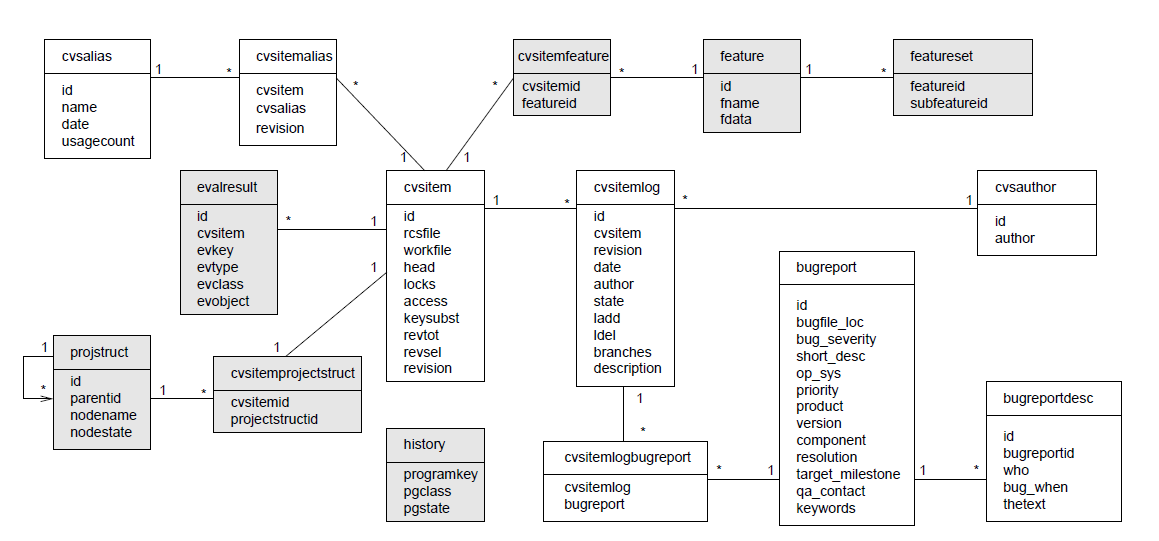
\includegraphics[width=0.8\textwidth]{images/rhdb_er}
	\caption{RHDB ER-Model \cite{fischer2003populating}}
	\label{fig:rhdber}
\end{figure*}

With this RHDB ER-Model it is possible to execute SQL-queries that can present a view on software evolution of the project. A sample query to list all bug reports for \textit{nsNSSDialogs.cpp}, presented by Fischer et al. is e.g. \cite{fischer2003populating}:

\begin{verbatim}
SELECT
	b.bugreport, r.bug_severity, r.short_desc
FROM
	cvsitem i, cvsitemlog l,
	cvsitemlogbugreport b, bugreport r
WHERE 	
	i.id = l.cvsitem
	AND l.id = b.cvsitemlog
	AND b.bugreport = r.id
	AND i.rcsfile REGEXP 'nsNSSDialogs.cpp';
	
\end{verbatim}

The application of the method on the Mozilla project stated that it was possible to link bug reports with version control data in an effective way \cite{fischer2003populating}. 

%Wie hat sich die Wissenschaft bis jetzt entwickelt?
%Wer hat welche Voraussetzungen geschaffen?
%Welche vergleichbaren Ergebnisse gibt es bisher?
%Welche Fragen sind noch offen?
%Warum reicht das bisher Getane noch nicht?
%Soll eine bestimmte These widerlegt oder bestätigt werden?
%Welche sind die wichtigen Veröffentlichungen? Was sagen sie zum Thema?

\newpage
\section{Objective and significance of the study}
\label{sec:objective}
This chapter describes the objective of this study. It furthermore explain the significance on project software evolution researches.

\subsection{Objective}

The objective of this study is to detect relations between the issues of a software project and how they
are related. To achieve this goal we try to develop an algorithm which is able to match the descriptions
of issues and the commit messages. To test and improve this algorithm we use the data of an real software
project until it turns out satisfactory. The results of the algorithm are evaluated by ourselves wherefore
a user study is strongly recommended.

\subsection{Significance}
The significance of this study become clear by viewing some scenarios:
Since most software systems consists of thousands lines of code it is really heavy for new new developers
to understand the existing code. There are multiple ways to help these developers to get into the code.
One option is a good documentation of the code. To improve the advantage taken by such a documentation it
should contain multiple diagrams and similar graphics describing the code.\\

Usually a software project is not documented as good as it should be that new programmers can understand
the existing code with low effort. Some documentations contain only a few graphics if there is a
documentation at all since the creation is very time-consuming. In order to save expenses the creation and
due the fact that the documentation has mostly just secondary importance the developers doesn't invest
enough time to create a proper documentation. Since creating graphics is a very time-consuming task,
especially when they won't be generated, most documentations have a lack of them.\\

New developers need to get an understanding how application works internally. Therefore they need to know
how the individual parts interact with each other. 
By matching issues with commit-messages new developers can see which changes are made to implement a new
feature by taking a look at the changed files. This is a time-consuming task, too. But the opportunity to
understand which changes are made to the code in order to add new functionality to the applications gives
the possibility to get an understanding how the code is designed. That's why using a software which
matches the issues with the commits allows a deeper understanding of the code.


\begin{figure}[H]
\centering
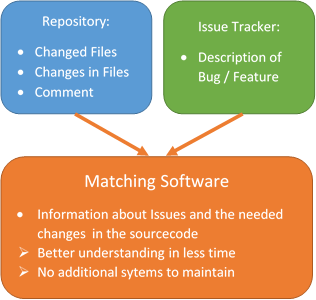
\includegraphics[width=0.5\textwidth]{MatchingUseCase.png}
\caption{Benefits from Matching}
\label{MatchingBenefits}
\end{figure}

The matching of issues and commits is independent of the creation of a documentation, yet it doesn't allow
to refrain it. Since most development teams work with any kind of version management software and a
software to track their bugs and issues they have all they need in order to use such a software as we
describe in this paper. In conclusion the developers don't need to install and maintain additional
software but they have the benefit of the matching. That means that they don't have any effort if they
just create comprehensive commit messages and issues.

\section{Methods}
\label{sec:methods}

\begin{figure*}[t]
  \centering
  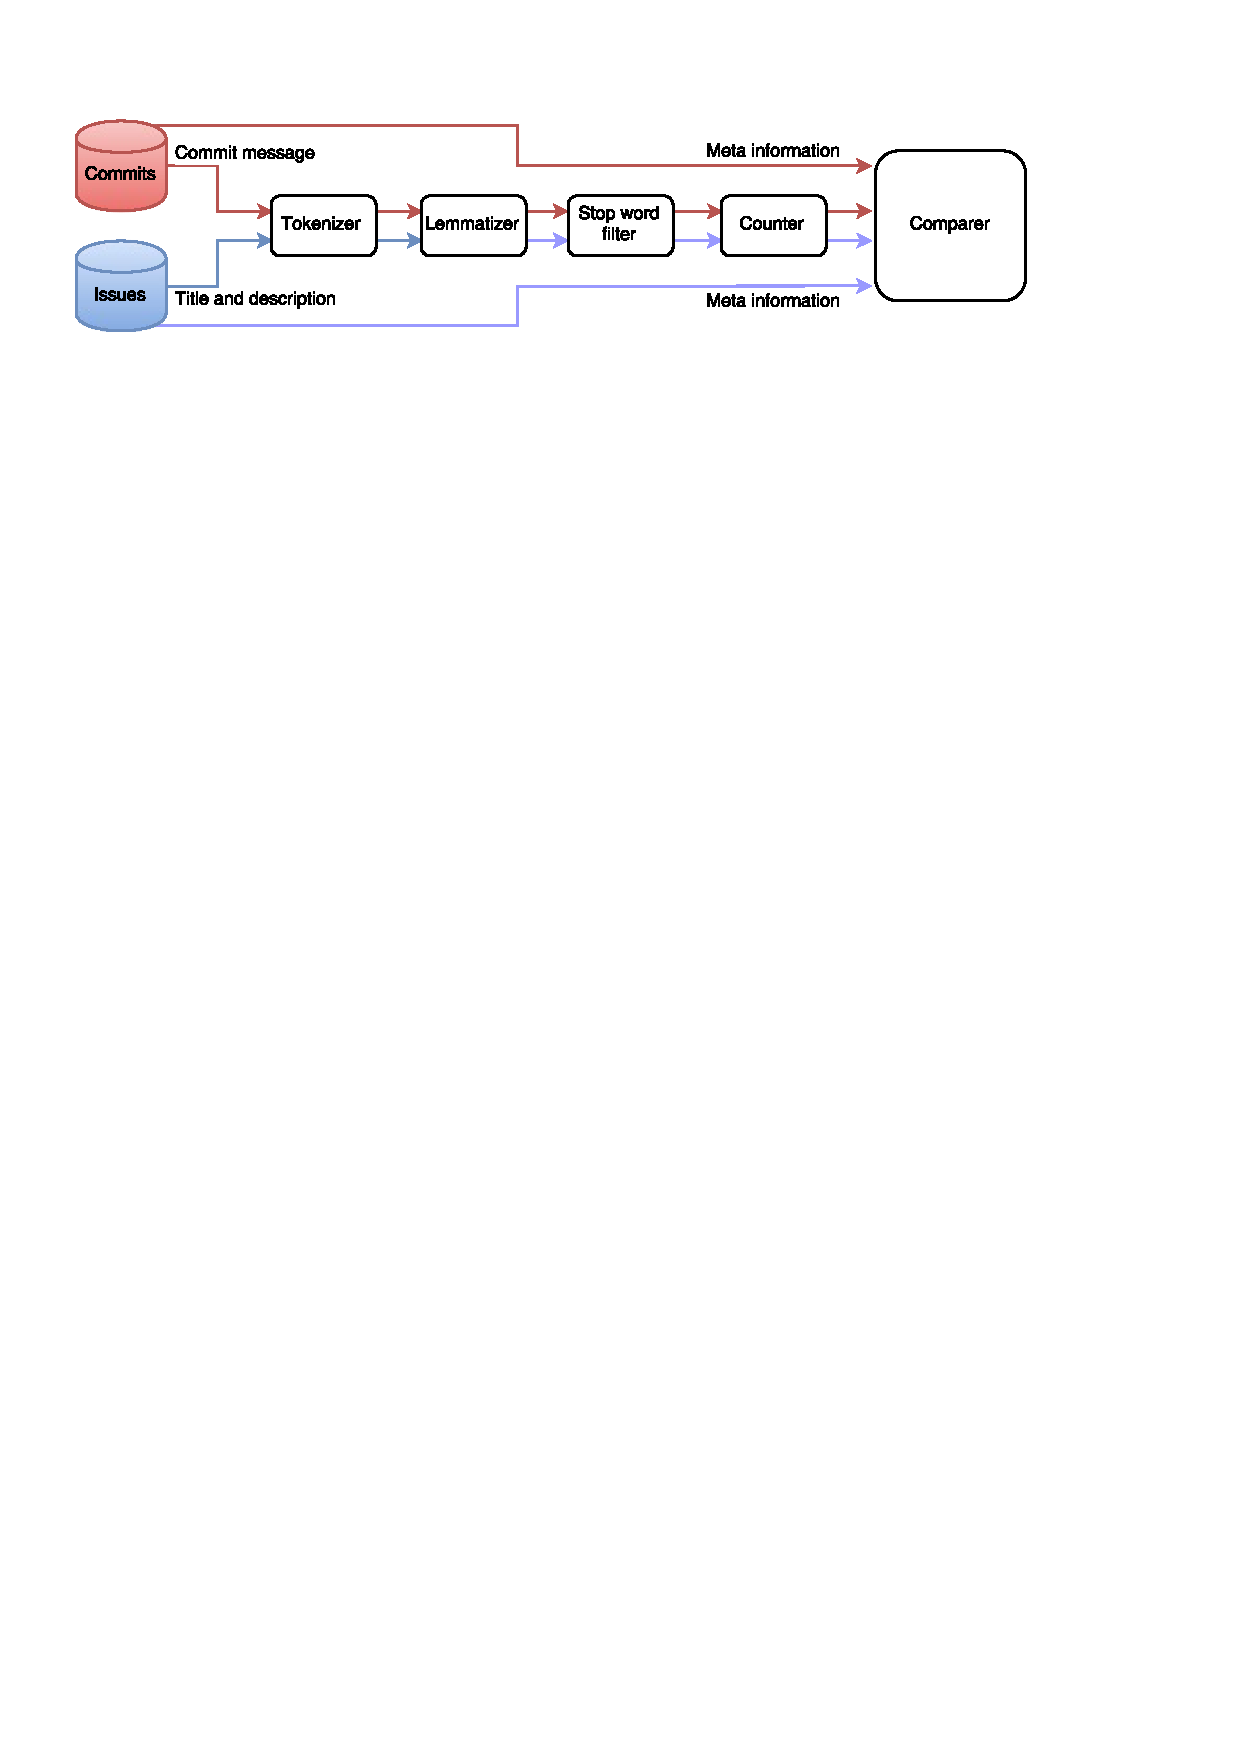
\includegraphics[width=\textwidth,trim={0 24cm 0 0},clip]{images/methods_vis.pdf}
  \caption{Pipeline of steps}
  \label{fig:methods_vis}
\end{figure*}

In order to find a relation between the commit messages and the issues, we need to start by reading the input data and tokenizing each commit message and the title and description of each issue into tokens.
In order to properly analyze natural languages, we need to lemmatize the tokens.
Lemmatization makes it possible to detect words that have the same meaning but appear differently in the text, either because of its tense (like ''walk'' and ''walked'') or because of the nature of that word (like ''good'' and ''better'').
Lemmatization normalizes every word so that we have one token for every word with the same meaning.
After the lemmatization step, we need to remove stop words so that only the interesting tokens are left.
The resulting tokens will then be placed in a table where the frequency of each token is stated for each commit message and issue.
Using this frequency table of tokens, we can compare the tokens of commit messages with the tokens of issues and find out the similarities based on the common tokens.
Figure \ref{fig:methods_vis} shows how these steps are to be processed one after another.


We also have access to the date, theme and the author for both commit messages and issues.
This kind of information can be useful when matching issues with commit messages.
For example, if a commit is done after an issue was submitted, it is less likely that the cause of this issue is related to that commit.
Similarly the theme and the author of commits and issues can help us classify the input and provide better results.
Grouping the commits and issues by their themes can increase the accuracy of matching and when the common words are not enough to determine a match, the system can provide a set of commits with a similar theme to the issue, instead of a single matching commit.
This might make it easier to find the commit manually, since the user has to only search a portion of the commits.

\subsection{Parsing}

\subsubsection{Parsing Issues}
Issues are provided as a .csv file, which is extracted from JIRA issue tracking system.
When we investigate the file, we realize that it follows the common .csv features and uses '';'' to separate the columns.
We have read and separated the values in our Java code and mapped it to an instance of our Issue class shown in Figure \ref{fig:issue}. 

\begin{figure}
\centering
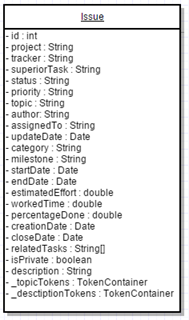
\includegraphics[scale=0.7]{issueClass}
\caption{Issue Java Class}
\label{fig:issue}
\end{figure}

One difference from a standard .csv format that the file exported from JIRA issue tracking system had was the additional description lines. Some issues have exception messages and log files attached to them to make it easier to describe the issue and provide further resources for the developer, who will fix the issue.
These descriptions contain multiple lines and thus a standard .csv parser cannot properly detect them.
Since the additional descriptions might be useful to understand more on what the issue is about, which is important for our case, we have implemented an additional functionality to detect these description lines and store them in our object.

We have created a regular expression shown in Figure \ref{fig:regexp} that detects whether a string is a new data record or not.

\begin{figure}
\centering
\verb/[0-9]+;[^\\n]+/
\caption{Regular Expression used to detect a new data record}
\label{fig:regexp}
\end{figure}

When reading each line of issue, we check the next line in the document before we move onto the next issue and we use the regular expression to determine whether this next line is a new issue or a line that contains additional description about the current issue.
If we detect additional description lines, then we also store them in the respective places in our java object.

Each issue object is then added to an ArrayList to store for further processing.

\subsubsection{Parsing Commits}

Commits are extracted from an SVN repository as a .txt file.
Each line in the file represents a single commit.
The information about the commit is separated by ''\#\#'' characters and each line is ended with ''\**'' characters.
Some commits also contain the duration of that particular task in the commit message, encoded by the ''@'' character followed by the time taken for that task.
An example line of commit can be seen in Figure \ref{fig:commitLine}.

\begin{figure}
\centering
\verb/4013453##Markt Benedikt##Thu Feb 20 04:39:35 2014##Delete Button Problem bei Links umgangen refs #803 @1h\**  /
\caption{An example line of commit}
\label{fig:commitLine}
\end{figure}

We have parsed each commit line in our Java program by separating them by ''\#\#'' characters, and then mapping them to an instance of our Commit Java class, shown in Figure \ref{fig:commit}.
We also detect the duration of each task by searching the ''@'' character inside the commit message.
The resulting Commit objects are then stored in an ArrayList for further processing.

\begin{figure}
\centering
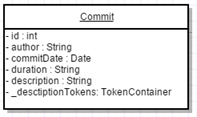
\includegraphics[scale=0.7]{commitClass}
\caption{Commit Java Class}
\label{fig:commit}
\end{figure}

\subsection{Tokenization}

When we set the description and the topic of an Issue object and the description of a Commit object, the input is immediately tokenized and stored in respective TokenContainer objects, which stores the tokens and their frequencies in a table like structure.

The tokenization process is done by separating each input text by whitespace characters.
The resulting words are stored in a TokenContainer and the TokenContainer is responsible for counting the frequencies of the words in the input text.
Later we can use the TokenContainer object to access every token and their frequencies.


\subsection{Lemmatization}

We use a library developed by Dr. Dipl. Inf. Ahmet Aker from University of Sheffield to do the lemmatization.
The library provides a functionality to determine the part-of-speech of a word and then it gives the lemma for that word given the correct part-of-speech.
The library has its own dictionary for part-of-speech tagging and lemmatization, and it supports English, German, Dutch, Spanish, Italian and French languages.

After getting the lemma for each word, we remove that token from our TokenContainer and instead insert the lemma as a new token.
This way different words that have the same lemma are counted as a single type of token and the frequency is also properly calculated.

There are other lemmatization libraries, e.g. OpenNLP or StanfordNLP, but most of these libraries only offer English lemmatizers.
Our commit messages and issue descriptions are mostly German, so we looked for a tool with support for the German language.
There are only few free tools available on the web and even less which support the required language.
That is why we decided to choose the previously described library.
Probably the results would be more accurate if we had English commit messages and issue descriptions and we could have used a more distributed NLP tool for lemmatization.


\subsection{Categorizing the issues and commits}

If an assignment of a issue to a commit is not possible one might want to think of another way for narrowing them down to a specific category or something similar.
This section describes some ideas for achieving a categorization of commits and issues in order to be able to support mapping them manually or at least summarize those which refer to a similar topic.

\subsubsection{Why categorization?}

It is difficult to explicitly map commits to issues.
One reason for that are the four different cases which have to be considered in this kind of mapping.\\

In case one the commit is mapped to only one issue which makes the mapping pretty simple.
The commit is mapped to a corresponding issue and both are not to be used in any further mapping.
This only applies if it is safe to assume that each commit addresses one specific issue which leads to the second case.\\

In the second case it is allowed that one commit might belong to several issues.
Although this case is usually quite rare it cannot be ignored.
For instance implementing a function which was defined in a issue could lead to improve efficiency of another functionality or anything similar which was described in another issue.
Obviously the commit would address to two different issues in this case.\\

The third case would be the other way around which means mapping several commits to one issue.
This case is probably the one which is to be considered the most.
In many cases it is not possible to resolve a problem stated in a issue within a short amount of time.
This results in interrupting the work on the issue and continue working on it on another time.
In this case it is inevitable to save the changes which were already made which usually happens by committing them.
It is now necessary to be able to gather all commits linked to this specific issue and map them accordingly.\\
\newpage
The last case deals with mapping several commits to several issues.
This case might not be seen as actual case since it can be separated into either the second and the third case.
This separation depends on whether the commits are supposed to be mapped to issues or the other way around.
The most common case would be mapping commits to issues.
In this case one could simply look at each single commit and map it to its corresponding issues (case two).
The other way would imply to look at each single issue mapping it to its corresponding commits.\\

These 4 cases illustrate that the affiliation of a specific commit to a specific issue is not always to be taken for granted.
This leads to another way of mapping commits and issues without having to explicitly map them to each other.
Instead one creates categories out of the token of the commits and issues and relates the commits and issues to the category they fit in whereby it is not specified that they can only be mapped to one category.

\subsubsection{Creating categories}

Having already tokenized and lemmatized the commits and the issues the basis for a categorization of these commits and issues is established.
Knowing how often a specific token (e.g. a specific word such as ''GUI'', ''bug'' or ''interface'') occurs, enables the creation of categories  depending on their occurrences.
It would be possible to map commits and issues which contain the word ''GUI'' to the corresponding category.
For designing this mapping process it is important to determine some restriction for creating categories as well as assigning commits and issues to them. 

\paragraph{Quantity of keywords}

In order to create a category we need to define a quantity of words referring to the same part of the software.
For instance in order to refer to the ''graphical user interface'' you could write about the ''GUI'' or about the ''front end''.
It is also possible to simple refer to it as ''user interface'' or ''UI''.
These mentioned words would be the quantity of words for the graphical user interface. \\

As you can see creating a category makes use of several (different) tokens which might be valid in several categories.
Assigning ''user interface'' to the category of the graphical user interface implies that the token ''interface'' is mapped to this category as well.
If a commit or issue now refers to another kind of ''interface'' such as ''library interface'' is it not possible to map it to a unique category.
This raises the question of how to handle this kind of overlapping. 

\paragraph{Frequency range and token summary}

On the one hand one could assume that words which are written next to each other (e.g. ''user'' and  ''interface'') have the same frequency within this issue with a deviation of 'x'.
The deviation is necessary because the token ''user'' could be referred to independent to the word ''interface''.
This also applies the other way around. \\

One the other hand this assumption does not guarantee an explicit mapping.
Considering the fact that categorizing issues and commits is only done if a specific mapping of them failed one should think about loosen the constraints.
In order to summarize several tokens to a single one the definition should not rely on the frequency itself and it should not aim to a specific mapping.
A loosened definition enables a summary of several words to a ''new token'' for the categorization which raises the chance of successfully mapping commits and issues.
In this case the user can optionally define a threshold for a frequency of a token which has to be met in order to be used for the creation of a new token and finally a new category.


\subsubsection{Mapping to categories}

Generally one would assume that a commit or issue which was mapped once cannot be mapped again.
This does not apply to mapping commits and issues to categories since a commit or issue can refer to several categories.
This depends on the created categories and cannot be defined generally.\\
This leads to mapping commits and issues to categories independent of them being already mapped.
Also the result or components of the previous mapping should influence further mappings.
The mapping itself depends on the categories and the tokens they were made of.
Basically all commits and issues which contain a token fitting into any category are mapped to it accordingly. \\

Concerning the mapping there are some tolerances which the user himself can adapt to his needs and preferences.
For instance the user can define a threshold for the frequency which has to be met in order to be mapped to a category.
This threshold might even be related to the threshold for the creation of the category itself. \\

The way of mapping commits and issues to a category as well as the way of creating those categories has many aspects which can be changed and adapted by the user.
They can depend on preferences, previous experiences or correlations between the token frequency.



\section{Implementation results}
\label{sec:implementation_results}
To test the algorithm described in \nameref{sec:methods} we implemented a prototype for associating commits from a version control system and issues from an issue tracking system.
We used real data from an academic software project to test different variants of the mapping algorithm.
In this section we describe the results we achieve with the sample data with different variants of the algorithm.

\subsection{Data requirements}
To achieve useful results it is important to have a reasonable data basis.
That means the issues need to describe the required task and do not just consist of a title, the commit messages need to describe the functional background and not the implementation details and, what is very important, the commit messages need to be in the same language as the issue descriptions.
In German projects a very common approach is to write the code documentation in English, this mostly includes the commit messages, too.
On the other hand the issue descriptions, the wiki entries, mailing lists etc. are often held in German.

\subsection{Our data basis}
We used the data from a real project, i.e. a students' academic project which took place at university Stuttgart in winter term 2013/14.
The data set contains 1107 commits and 500 issues.
The commit messages mostly start with a reference number to link with an issue.
Of course we did not use them to match the commit to that issue, but we used them to check our results.
The issue descriptions are mostly in German, whereas the commit messages are partly German and partly English.
This led to problems, as only the German commit messages could be used.
But the biggest problem originated from the commit messages themselves.
The project members mostly described the technical background instead of providing a functional description of what they did.
As the issue descriptions did not prescribe the implementation details, the words used in the commit message and that given in the issue description usually differed.
For example one project member often started his commit messages with the issue reference number, followed by the word ''Erledigt'', which means ''Done''.
After that he described how he implemented the feature.
For instance he names hotkeys he used for activating the feature.


\section{Summary}
\label{sec:summary}
We have described a method for connecting commits and issues by comparing their commit messages, titles and descriptions as well as by having a look at the meta information of issues and commits.
If the assignment of an issue to a commit is not possible, we propose a categorization of the issues and commits for supporting at least a less accurate mapping to categories.
We then implemented a prototype to test our theories by using real data from an academic software project and we came to the conclusion that our method generally works fine but only if we improve the quality of the commit messages.
In our original sample data the messages were too inaccurate and mainly because of this we were not able to link many commits to their related issue.\\
A possible approach in the future is to scientifically refine the method by studying several software projects to find the best balance within the rating parameters and for example by finding a way to be more tolerant with commit messages, which do not follow best practices.
One then can expand the prototype to a customizable software one can use for issue and commit logs, regardless of the original format and with adjustable rating parameters with the help of an interactive user interface.

%\end{document}  % This is where a 'short' article might terminate



%
% The following two commands are all you need in the
% initial runs of your .tex file to
% produce the bibliography for the citations in your paper.
\bibliographystyle{abbrv}
\bibliography{bibliography}  % sigproc.bib is the name of the Bibliography in this case
% You must have a proper ".bib" file
%  and remember to run:
% latex bibtex latex latex
% to resolve all references
%
% ACM needs 'a single self-contained file'!
%
%APPENDICES are optional
%\balancecolumns

%\appendix
%Appendix A
\section{Headings in Appendices}
The rules about hierarchical headings discussed above for
the body of the article are different in the appendices.
In the \textbf{appendix} environment, the command
\textbf{section} is used to
indicate the start of each Appendix, with alphabetic order
designation (i.e. the first is A, the second B, etc.) and
a title (if you include one).  So, if you need
hierarchical structure
\textit{within} an Appendix, start with \textbf{subsection} as the
highest level. Here is an outline of the body of this
document in Appendix-appropriate form:
\subsection{Introduction}
\subsection{The Body of the Paper}
\subsubsection{Type Changes and  Special Characters}
\subsubsection{Math Equations}
\paragraph{Inline (In-text) Equations}
\paragraph{Display Equations}
\subsubsection{Citations}
\subsubsection{Tables}
\subsubsection{Figures}
\subsubsection{Theorem-like Constructs}
\subsubsection*{A Caveat for the \TeX\ Expert}
\subsection{Conclusions}
\subsection{Acknowledgments}
\subsection{Additional Authors}
This section is inserted by \LaTeX; you do not insert it.
You just add the names and information in the
\texttt{{\char'134}additionalauthors} command at the start
of the document.
\subsection{References}
Generated by bibtex from your ~.bib file.  Run latex,
then bibtex, then latex twice (to resolve references)
to create the ~.bbl file.  Insert that ~.bbl file into
the .tex source file and comment out
the command \texttt{{\char'134}thebibliography}.
% This next section command marks the start of
% Appendix B, and does not continue the present hierarchy
\section{More Help for the Hardy}
The sig-alternate.cls file itself is chock-full of succinct
and helpful comments.  If you consider yourself a moderately
experienced to expert user of \LaTeX, you may find reading
it useful but please remember not to change it.
%\balancecolumns % GM June 2007
% That's all folks!

\end{document}
